%%%% Proceedings format for most of ACM conferences (with the exceptions listed below) and all ICPS volumes.
\documentclass[sigconf]{acmart}

% \usepackage{amsmath}
%%%% As of March 2017, [siggraph] is no longer used. Please use sigconf (above) for SIGGRAPH conferences.

%%%% Proceedings format for SIGPLAN conferences 
% \documentclass[sigplan, anonymous, review]{acmart}

%%%% Proceedings format for SIGCHI conferences
% \documentclass[sigchi, review]{acmart}

%%%% To use the SIGCHI extended abstract template, please visit
% https://www.overleaf.com/read/zzzfqvkmrfzn

%%
%% \BibTeX command to typeset BibTeX logo in the docs
\AtBeginDocument{%
  \providecommand\BibTeX{{%
    \normalfont B\kern-0.5em{\scshape i\kern-0.25em b}\kern-0.8em\TeX}}}

%% Rights management information.  This information is sent to you
%% when you complete the rights form.  These commands have SAMPLE
%% values in them; it is your responsibility as an author to replace
%% the commands and values with those provided to you when you
%% complete the rights form.
\setcopyright{acmcopyright}
\copyrightyear{2019}
\acmYear{2019}
\acmDOI{10.1145/1122445.1122456}

%% These commands are for a PROCEEDINGS abstract or paper.
% \acmConference[DocEng '19]{DocEng '19: ACM Symposium on Document Engineering}{September 23--26, 2019}{Berlin, DE}
% \acmBooktitle{Woodstock '18: ACM Symposium on Neural Gaze Detection, June 03--05, 2018, Woodstock, NY}
% \acmPrice{15.00}
% \acmISBN{978-1-4503-9999-9/18/06}


%%
%% Submission ID.
%% Use this when submitting an article to a sponsored event. You'll
%% receive a unique submission ID from the organizers
%% of the event, and this ID should be used as the parameter to this command.
%%\acmSubmissionID{123-A56-BU3}

%%
%% The majority of ACM publications use numbered citations and
%% references.  The command \citestyle{authoryear} switches to the
%% "author year" style.
%%
%% If you are preparing content for an event
%% sponsored by ACM SIGGRAPH, you must use the "author year" style of
%% citations and references.
%% Uncommenting
%% the next command will enable that style.
%%\citestyle{acmauthoryear}

%%
%% end of the preamble, start of the body of the document source.
\begin{document}

%%
%% The "title" command has an optional parameter,
%% allowing the author to define a "short title" to be used in page headers.
\title{Automatic Identification and Normalisation of Physical Measurements in Scientific Literature}

%%
%% The "author" command and its associated commands are used to define
%% the authors and their affiliations.
%% Of note is the shared affiliation of the first two authors, and the
%% "authornote" and "authornotemark" commands
%% used to denote shared contribution to the research.
\author{Luca Foppiano}
\email{FOPPIANO.Luca@nims.go.jp}
\orcid{0000-0002-6114-6164}
\affiliation{%
  \institution{National Institute for Materials Science (NIMS)}
  \streetaddress{1-2-1 Sengen}
  \city{Tsukuba}
  \postcode{305-0047}
  \country{Japan}
}

\author{Laurent Romary}
\email{laurent.romary@inria.fr}
\orcid{0000-0002-0756-0508}
\affiliation{%
  \institution{Inria}
  \streetaddress{2 Simone Iff}
  \city{Paris}
  \postcode{75012}
  \country{France}
}

\author{Masashi Ishii}
\email{ISHII.Masashi@nims.go.jp}
\orcid{0000-0003-0357-2832}
\affiliation{%
  \institution{National Institute for Materials Science (NIMS)}
  \streetaddress{1-2-1 Sengen}
  \city{Tsukuba}
  \postcode{305-0047}
  \country{Japan}
}

\author{Mikiko Tanifuji}
\email{TANIFUJI.Mikiko@nims.go.jp}
\orcid{000-0001-5284-6364}
\affiliation{%
  \institution{National Institute for Materials Science (NIMS)}
  \streetaddress{1-2-1 Sengen}
  \city{Tsukuba}
  \postcode{305-0047}
  \country{Japan}
}

%%
%% By default, the full list of authors will be used in the page
%% headers. Often, this list is too long, and will overlap
%% other information printed in the page headers. This command allows
%% the author to define a more concise list
%% of authors' names for this purpose.
\renewcommand{\shortauthors}{Foppiano, et al.}

%%
%% The abstract is a short summary of the work to be presented in the
%% article.
\begin{abstract}
We present Grobid-quantities, an open source application for parsing and normalising measurements from scientific and patent literature (\cite{grobid-quantities}). Tools of this kind represent the building blocks for large-scale Text and Data Mining (TDM) systems whose goal is to understand and make unstructured information accessible through standardised methods. 
Grobid-quantities is a module built up on top of Grobid (\cite{GROBID}), a machine learning framework for parsing and structuring PDF documents. Designed to process large quantities of data, it provides a robust implementation in batch mode or via a REST API. 
The machine learning engine architecture follows the cascade approach where each model is specialised in the resolution of a specific task. The models are trained using CRF (Conditional Random Field) algorithm for extracting quantities (atomic values, intervals or lists), units (like length, weight) and different value representations (such as alphanumeric, power of 10, exponential). Identified measurements are then normalised toward the International System of Units (SI) (\cite{internationalSystemOfUnits}). 
Thanks to its high recall and reliable precision, Grobid-quantities has been integrated as a measurement-extraction engine in various TDM projects, such as Marve (Measurement Context Extraction from Text) (\cite{hundman2017measurement}), for extracting semantic measurements and meaning in Earth Science. 
At the National Institute for Materials Science (NIMS), a project for application of Grobid-quantities to discover new superconducting materials is in progress: normalised materials characteristics extracted from scientific literature are a key resource for materials informatics (MI) (\cite{foppiano2019proposal}). 
\end{abstract}

%%
%% The code below is generated by the tool at http://dl.acm.org/ccs.cfm.
%% Please copy and paste the code instead of the example below.
%%
 \begin{CCSXML}
<ccs2012>
<concept>
<concept_id>10010405.10010497.10010504.10010505</concept_id>
<concept_desc>Applied computing~Document analysis</concept_desc>
<concept_significance>500</concept_significance>
</concept>
<concept>
<concept_id>10010405.10010497.10010500.10010503</concept_id>
<concept_desc>Applied computing~Document metadata</concept_desc>
<concept_significance>300</concept_significance>
</concept>
<concept>
<concept_id>10010405.10010497.10010510.10010514</concept_id>
<concept_desc>Applied computing~Format and notation</concept_desc>
<concept_significance>300</concept_significance>
</concept>
</ccs2012>
\end{CCSXML}

\ccsdesc[500]{Applied computing~Document analysis}
\ccsdesc[300]{Applied computing~Document metadata}
\ccsdesc[300]{Applied computing~Format and notation}

%%
%% Keywords. The author(s) should pick words that accurately describe
%% the work being presented. Separate the keywords with commas.
\keywords{machine learning, tdm, measurements, physical quantities}

%%
%% This command processes the author and affiliation and title
%% information and builds the first part of the formatted document.
\maketitle

\section{Introduction}

The data overflow in scientific publications is a widely known challenge impacting the accessibility to relevant information for both researchers and readers. Moreover, the amount of data a single scientists might be dealing with, risk of becoming overwhelming because understanding requires to spend many hours (re-)reading a single article to grasp its message and significance. In knowledge acquisition it's simply too much for a single human to keep up with the new fresh information that are available daily. 
Luckily technology has evolved: advances in natural language processing (NLP) in combination with Deep Neural Network have reached results above average human precision. 

%Motivation
When observing the content produced in scientific literature, it's emerging that many technical fields deliver key information in the form of figures and quantitative information. While figures requires particular processing, quantitative information can be decoded with special approaches in order to obtain highly valuable structured information. Physical quantities are also relatively central information, shared among several domains. In an attempt to model such concept, we can consider measurements as composed by a quantified amount referring to an (optional) unit and measured object or substance (optional as well). 
There are, though, several challenges that are posed: (1) the variability of expressions is still "polluted" by the variability introduced by natural language, together with the writing style of the single author. (2) the standardisation cover only part of the expression that are used (for example length can be expressed as m, meter, metre). Lastly and more critical are the overlap (3) between different unit of measurements (such as pico Henry \textit{pH} and acidity to make an example). The ability extract and label measurements correctly, enable the creation of knowledge bases as ignition phase to foster text and data mining processes aiming to creating advanced semantic services. 

%Grobid-quantities
In this paper we present Grobid-quantity, an Open Source application \cite{grobid-quantities} for parsing and normalising measurements from scientific and patent literature. Using the machine learning (ML) CRF (Conditional Random Field) algorithm provides a framework for extracting quantities (atomic values, ranges, intervals and lists), units (like length, weight) and different value representations (such as alphanumeric, power of 10, exponential). Identified measurements are then normalised or transformed to the International System of Units (SI). Thanks to its high recall and reliable precision, Grobid-quantities has been integrated as a measurement-extraction engine in various TDM projects \cite{foppiano2019proposal}.

The article is organised as follow. In Section \ref{sec:related_work} we discuss other system for measurement extraction and normalisation. After, in section \ref{sec:system} we describe how the system work, the uses cases where it has been used (Section \ref{sec:use_cases}). In Section \ref{sec:conclusion} we conclude the paper and discuss prospects and future work. 

\section{Related Work}
\label{sec:related_work}
Previous attempts have been made to extract such data automatically from text, several of them related to patent literature. The majority relay on rule-based or formal grammar, combining handwritten rules with lookups on dictionaries of terms.  

% The most recent work of evaluation is provided by \cite{hundman2017measurement} which provides a rather detailed comparison of Grobid-quantities to other systems. 
A known commercial tool, Quantalyze, which, probably due to rule-based approach, tests resulted weak recall \cite{hundman2017measurement} covering a rather lower set of units \cite{aras2014applications}. Another tentative approach using GATE (General Architecture for Text Engineering) is described in \cite{agatonovic2008large} addressed in a sub-task for identifying numeric properties from patents. \cite{am2013processing} investigates issues applied to Russian-derived languages. These approaches lack either the generalisation to an extensive corpus or deal mainly with the specific languages. \cite{berrahou2013extract} described an attempt using machine learning algorithm in combination with pattern matching and distance measurement against an ontology to extract units. \cite{kang_extracting_2013} describe another ML-based approach focusing on experimental results restricted to biological domain, on which quantification of units is just a part of it. 
Our work recognise not only units but also quantitative values in various forms (atomic, list, ranges and intervals). Recognised entities are parsed and normalised to the International System of Units (SI). We have an additional module for recognising the quantified object or substance which, however, will be discussed in a following article.

\section{System description}
\label{sec:system}

In this section we describe how the system has been designed, we begin illustrating the data model used to carry out our representation of the problem. Further section explain the machine learning architecture, which models are created and how they are used. This section is then concluded with a detailed description of the normalisation process.

\subsection{Data model}
\label{subsub:data-model}
Before discussing in detail the functioning of the system, we delineate the abstract model of the measurement and physical quantities can be represented. 
The "entry point" is the concept of \textit{Measurement} composed by a \textit{type} and one or more \textit{quantities}. We have identified three type of measurements: (a) atomic, in case of a punctual measurement (10 grams). (b) interval (\textit{from 3 to 5 mmol}) and (c) range ($100 \pm 4$), when the quantification covers a continuous range of values. Finally, (d) conjunction representing discrete value of the same quantity. 

A quantity is the association between a value and an (optional) unit. See in Figure~\ref{fig:data-model-schema-2}, since we cover also enumeration, it's possible not to have a unit. Finally \textit{Value} and \textit{Unit} are expected to appear as \textit{raw}, when they are represented as appearing in text, \textit{parsed} when the numeric values are recognised or converted as such and finally, normalised which consists in finding the SI base unit by transforming (when in the same System) or computed (when from another system, for example from imperial miles to meters). 

\begin{figure}[h]
  \centering
  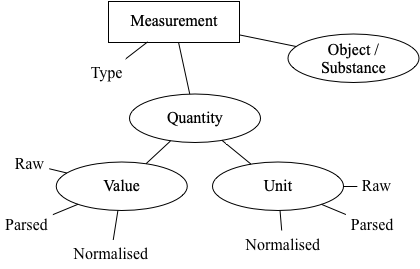
\includegraphics[width=\linewidth]{images/schema-2}
  \caption{Data model schema}
  \label{fig:data-model-schema-2}
  \Description{Data model schema}
\end{figure}

The idea behind this design, since the data we are dealing is noisy (spaces, wrong UTF-8 characters, missing fonts), is to provide a representation that allows to complete the process of extraction even with partial results.

We have designed \textit{Units} and \textit{Values} in order to support multiple representations. Values can be of five types: numeric (2, 1000), alphanumeric (two, thousand), power of 10 ($3\cdot10\textsuperscript{5}$) and exponential representation using the mathematical constant e = 2.2718 ($0.2\cdot e\textsuperscript{3}$), finally dates are also expressions of measurements of time. 

\textit{Units} are more complex to manage. In case of non-SI units, often but not always, be converted to their SI equivalent (like for example converting miles to meters). In case of SI units can be represented as products of units, for example m/s can be rewritten as $m \cdot s\textsuperscript{-1}$. Unit products are cleaner and can be easily normalised to their base unit.  

\subsection{Architecture}

Grobid-quantity architecture is composed by two phases: (a) extraction and parsing and (b) normalisation. As mentioned previously, the process has been designed to carry on until the end, and, in case of errors or mistakes, return partial data. For example if a number cannot be parsed, because of a invalid character, the parsed value will be null, and the client, once noticed that, can apply additional processing on the raw data. 


\subsubsection{Extraction}
The extraction is composed by three CRF (Conditional Random Field) models applied in cascade according to the schema in Figure \ref{fig:schema-cascade}: Quantities, Units and Values models. 

\begin{figure}[h]
  \centering
  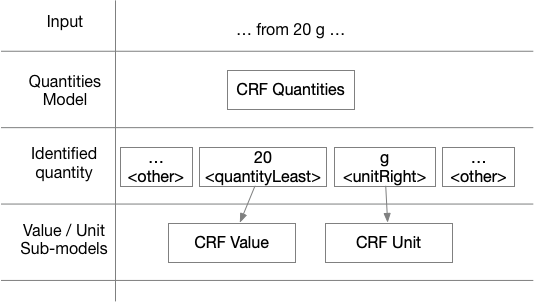
\includegraphics[width=\linewidth]{images/schema-cascade}
  \caption{Illustrate the cascade approach in applying CRF models. The input is first parsed by the quantities model, which recognise the type of measurement (list, ranges, interval and atomic values) and units. They are then passed to further CRF sub-models: in this case Value and Unit respectively.}
  \label{fig:schema-cascade}
  \Description{Illustrate the cascade approach in applying CRF models. The input is first parsed by the quantities model, which recognise the type of measurement (list, ranges, interval and atomic values) and units. They are then passed to further CRF sub-models: in this case Value and Unit respectively.}
\end{figure}

% Quantity model 

The \textit{quantities model} takes in input a raw text and apply text labelling using the six labels as illustrated in Table \ref{tab:quantities-model-labels}. This model is responsible to identify units and values and group them together. Because of that and  output from sequence labelling is flatten out, there is need of additional labels (such as two unit labels <unitLeft>, <unitRight>). 

\begin{table}
  \caption{Labels description for the CRF model for Quantities. In bold the token the label refers to.}
  \label{tab:quantities-model-labels}
  \begin{tabular}{lll}
    \toprule
    Label & Description & Example\\
    \midrule
    <valueAtomic> & value of an atomic quantity & \textbf{2} m \\
    <valueLeast> & least value in an interval & from \textbf{2} m \\
    <valueMost> & max value in an interval & up to \textbf{7} m \\
    <valueBase> & base value in a range & $\textbf{20}\pm7$ m \\
    <valueRange> & range value in a range & $20 \pm \textbf{7}$ m \\
    <valueList> & list of quantities & \textbf{2}, \textbf{3} and \textbf{10} m \\
    <unitLeft> & left-attached unit & \textbf{pH} 2 \\
    <unitRight> & right-attached unit & 2 \textbf{m} \\
    <other> & everything else & - \\
  \bottomrule
\end{tabular}
\end{table}

The quantity model works at token level, where each token is generated by splitting the input by almost any kind of punctuation and space. Numeric expressions such as 2.5 m are also split in ["2",".","5"," ","m"]. The model uses only standard lexical features, it does not use layout information such as formatting, subscript or superscript. 
To improve the recognition we provide the model two additional features result of the lookup on two gazetteers: list of units and their representation such as notations (m), lemmas (meter or metre) and inflections (meters, metres). The second gazetteer is a generated list of alphabetic values (twenty-one, etc.). These gazetteers are in English, French and German. 

% Unit model 
The unit model is applied to every token identified as unit. This model works at character level and is applied to every entities recognised as Unit from the Quantity model. They are segmented in product of triples (prefix, base, power) as they are modelled in the SI system (Table \ref{tab:units-model-labels}). This approach is very convenient to parse complex units. For example Kg/mm\textsuperscript{2} can be rewritten as [(K, g, 1),(m, m, -2)]. This model is compatible with unit outside SI, for example for an imperial unit like \textit{mile} can be recognised entirely as a single product of a base, like [(,mile,)].

\begin{table}
  \caption{Labels description for the CRF model for Units. }
  \label{tab:units-model-labels}
  \begin{tabular}{lll}
    \toprule
    Label & Description & Example\\
    \midrule
    <prefix> & prefix of the unit  & \textbf{k}g\textsuperscript{2} \\
    <base> & least value in the quantity & k\textbf{g}\textsuperscript{2}\\
    <pow> & max value in the quantity & kg\textsuperscript{\textbf{2}}\\
    <other> & everything else & - \\
  \bottomrule
\end{tabular}
\end{table}

Once the units are segmented, we reformat them and perform a lookup in our unit gazetteer to retrieve all complementary information, like system, type. For example, suppose the text contains "10 m 3". The Quantity model identify 10 as atomic value and "m 3" as unit. The Unit model identify "m" as base and "3" as power, the unit is then reformatted as "m\^2" and looked up in the gazetteer. Since "m\^3" represent a complex unit "Cubic meters" is found and information like type /textit{volume} and system SI Base are attached to to the unit. 

% Value model 
The value model processes the values recognised by the Quantities model in five type of expressions: numeric, alphabetic, power-10, exponential, and time expression using the labels defined in Table \ref{tab:values-model-labels}). This model is crucial to support multiple value expression used in natural language and apply the correct parser: alphabetic expression are looked up on a word-number converter, power-10 and exponential are parsed and the total is calculated. Time expression are processed using the built-in Date model from Grobid \cite{GROBID}.

\begin{table}
  \caption{Labels description for the CRF model for Values. In bold an example of token the specific label recognise.}
  \label{tab:values-model-labels}
  \begin{tabular}{lll}
    \toprule
    Label & Description & Example\\
    \midrule
    <number> & numeric value & $\textbf{2.5}\cdot10\textsuperscript{\textbf{5}}$ \\
    <alpha> & alphabetic value & \textbf{twenty} \\
    <time> & time expression  & in \textbf{1970-01-02}\\
    <exp> & exponential expression & $0.2\cdot\textbf{e}\textsuperscript{3}$ \\
    <base> & base of the power expression & $2.5\cdot\textbf{10}\textsuperscript{5}$\\
    <pow> & power in a power expression & $2.5\cdot10\textsuperscript{\textbf{5}}$ \\
    <other> & everything else & - \\
  \bottomrule
\end{tabular}
\end{table}

\subsubsection{Normalisation}

The normalisation is the last step of this process. All the measurement that have been parsed correctly are then eligible for normalisation. To perform this task we have selected an external library called Unit of Measurement. Units of Measurement provides a set of APIs and services for handling units and quantities; developed in Java as the succession of the JMeasurement library has been standardised 


\subsubsection{Service}
\section{Use cases}
\label{sec:use_cases}
\subsection{ISTEX}
\subsection{NIMS}
\subsection{Marve}
\section{Conclusion}
\label{sec:conclusion}

%%
%% The acknowledgements section is defined using the "acks" environment
%% (and NOT an unnumbered section). This ensures the proper
%% identification of the section in the article metadata, and the
%% consistent spelling of the heading.
\begin{acks}
We would like to address our warmest thanks to Patrice Lopez, who initially started developing Grobid-quantities. Patrice is also the author of Grobid~\cite{GROBID} (GeneRation Of BIbliographic Data), \textit{entity-fishing} and many other TDM tools for scientific literature. 
\end{acks}

%%
%% The next two lines define the bibliography style to be used, and
%% the bibliography file.
\bibliographystyle{ACM-Reference-Format}
\bibliography{references}

%%
%% If your work has an appendix, this is the place to put it.
% \appendix

\end{document}
\endinput
%%
%% End of file `sample-sigconf.tex'.
